\part{Ejecución: Infraestructura Base y Entorno}

\chapter{Introducción Técnica al Entorno de Desarrollo}

Esta fase establece la orquestación inicial del monorepositorio utilizando espacios de trabajo (\textit{npm workspaces}) para unificar el desarrollo del cliente (\textit{Vite/React}) y el servidor (\textit{Node.js/Express}). La arquitectura se basa en contenedores \textit{Docker}, permitiendo un despliegue aislado de los servicios de infraestructura (\textit{MariaDB} y \textit{Redis}) para garantizar la paridad de entornos locales y facilitar la futura integración continua.

\textbf{Estructura de Directorios} \\
\begin{verbatim}
KingAndPeasant/
|-- docker-compose.yml
|-- packages/
|  |-- client/
|  |  |-- src/
|  |  +-- package.json
|  +-- server/
|     |-- src/
|     +-- package.json
+-- package.json
\end{verbatim}

\chapter{Iteración 1: Configuración de Entornos, Planificación Inicial y Metodología Base}

\section{Definición de Características}
El objetivo primordial de esta primera iteración consiste en establecer los cimientos arquitectónicos e infraestructurales del proyecto \textit{King and Peasant}. A su vez, otro de los principales objetivo es establecer los cimientos organizativos del proyecto, preparando las herramientas de planificación e inicializando las metodologías de trabajo colaborativo. Las tareas principales consisten en la configuración inicial del entorno de trabajo del proyecto, la creación del calendario inicial de desarrollo y la redacción del documento de metodología para el uso de GitHub. A continuación, se detalla el contenido y el propósito de cada elemento:

\begin{itemize}
    \item \textbf{Configuración inicial del proyecto:} Se busca orquestar un entorno de desarrollo basado en un monorepositorio mediante \textit{npm workspaces}, permitiendo la gestión unificada del cliente (\textit{Vite/React}) y el servidor (\textit{Node.js}). Para garantizar la paridad entre los entornos de los distintos desarrolladores, se define la contenedorización de los servicios de infraestructura crítica, específicamente \textit{MariaDB} para la persistencia relacional y \textit{Redis} para el estado volátil en memoria. Asimismo, se pretende automatizar el flujo de arranque local integrando herramientas de ejecución concurrente que coordinen el despliegue de migraciones, la generación del cliente de base de datos y la inicialización sincronizada de los servicios de aplicación.
    \item \textbf{Calendario inicial de desarrollo:} Consiste en la elaboración de un cronograma estructurado que distribuye temporalmente los elementos del alcance del proyecto. En este documento se estiman los tiempos necesarios para implementar los distintos módulos, integrando el desarrollo de la lógica, la conexión entre sistemas y la redacción de la memoria. Lo que se busca con esta planificación es establecer una línea base que permita monitorizar el progreso real frente al esperado. El sentido de este calendario es identificar posibles desviaciones de tiempo de manera temprana, equilibrar la carga de trabajo a lo largo de las semanas y garantizar que el trabajo finaliza dentro de los plazos académicos establecidos.
    \item \textbf{Documento de metodología para el uso de GitHub:} Se trata de una guía interna que estipula las normas de control de versiones que se aplican durante todo el ciclo de vida del software. Su propósito fundamental es evitar conflictos en el código al trabajar de manera simultánea y asegurar que la evolución del proyecto quede documentada de forma ordenada. Este documento define tres pilares esenciales:
    \begin{itemize}
        \item \textbf{Gestión de ramas (\textit{branches}):} Se establece una estructura que aísla los entornos. Se define cómo y cuándo se crean ramas independientes para desarrollar nuevas funcionalidades antes de integrarlas al proyecto principal. El objetivo es asegurar que la rama principal contenga siempre código estable y funcional.
        \item \textbf{Gestión de \textit{issues}:} Se instaura el uso de \textit{issues} como sistema unificado para el registro de tareas pendientes, seguimiento de errores e implementación de nuevas características. El sentido de esta práctica es mantener un control centralizado del trabajo pendiente y facilitar la asignación equitativa de tareas.
        \item \textbf{Nomenclatura de \textit{commits}:} Se fijan reglas estrictas para la redacción de los mensajes de confirmación de cambios en el repositorio. Lo que se busca es que cada modificación en la base de código sea descriptiva y fácilmente comprensible por ambos integrantes. Esto resulta vital para mantener la trazabilidad del desarrollo, identificar rápidamente cuándo se introdujo un cambio específico y facilitar la resolución de problemas si es necesario revertir una versión.
    \end{itemize}
\end{itemize}

\section{Diseño de la Solución}
Para abordar estas características, el diseño se articula en torno a la orquestación inicial del entorno. A nivel de equipo, se diseña una estructura de monorepositorio y se redacta el documento de metodología en Markdown para estandarizar el flujo de trabajo (ramas, \textit{commits} y seguimiento de \textit{issues}). A nivel técnico, para satisfacer el requisito de arquitectura (\textbf{RNF-ARQ}), el diseño contempla el uso de \textit{Docker} y \textit{Docker Compose}. La creación de los archivos \texttt{Dockerfile} permitió plantear un despliegue aislado de los entornos de ejecución base (véase la Fig.~\ref{fig:docker_topology}).

\begin{figure}[H]
\centering
\begin{tikzpicture}[
    scale=0.7, transform shape,
    node distance=2.5cm,
    service/.style={rectangle, draw=ThemeColor1, fill=ThemeColor2, thick, minimum width=3cm, minimum height=1.2cm, align=center, rounded corners},
    infra/.style={cylinder, draw=ThemeColor1, fill=ThemeColor2, thick, minimum width=2cm, minimum height=1.5cm, shape border rotate=90, align=center},
    network/.style={draw=ThemeColor1, dashed, thick, inner sep=0.8cm, rounded corners}
]
    \node[service] (client) {Client \\ \small (Vite/React)};
    \node[service, right=of client] (server) {Server \\ \small (Node.js/Express)};
    \node[infra, below=1.5cm of server, xshift=-1.5cm] (mariadb) {MariaDB \\ \small (Relational)};
    \node[infra, below=1.5cm of server, xshift=1.5cm] (redis) {Redis \\ \small (In-Memory)};
    \draw[<->, >=stealth, thick, ThemeColor1] (client) -- node[above, black] {\scriptsize HTTP/WS} (server);
    \draw[->, >=stealth, thick, ThemeColor1] (server) -- node[left, black, xshift=-0.1cm] {\scriptsize SQL} (mariadb);
    \draw[->, >=stealth, thick, ThemeColor1] (server) -- node[right, black, xshift=0.1cm] {\scriptsize Events} (redis);
    \begin{pgfonlayer}{background}
        \node[network, fit=(client) (server) (mariadb) (redis), label={[ThemeColor1]above:Docker Internal Bridge Network}] {};
    \end{pgfonlayer}
\end{tikzpicture}
\caption{Diagrama de topología de contenedores de la infraestructura base, ilustrando la red interna (bridge) entre el servidor, MariaDB y Redis.}
\label{fig:docker_topology}
\end{figure}

Por otro lado, el calendario inicial se diseña mediante la herramienta Obsidian para proporcionar una hoja de ruta clara de las tareas a realizar. Este se estructura en iteraciones de una semana, priorizando inicialmente la configuración y tareas sencillas para facilitar la toma de contacto con las tecnologías, dejando la lógica central para la fase media y un periodo final dedicado exclusivamente a pruebas y corrección de errores. Por otro lado, la metodología de GitHub se diseña para garantizar un desarrollo conjunto organizado, definiendo roles específicos para cada rama y reglas estrictas de integración de código que materializan la mitigación planificada frente al riesgo de conflictos en el repositorio (\textbf{RO-03}, véase la Tab.~\ref{tab:matriz_riesgos}).

\section{Detalles de Implementación}
Para asegurar la cohesión del monorepositorio, se estructura el proyecto utilizando \textit{npm workspaces}, agrupando el cliente (\textit{Vite/React}) y el servidor (\textit{Node.js}) bajo un único árbol de dependencias. La orquestación se materializa a través de \textit{scripts} centralizados en el \texttt{package.json} raíz, combinando \textit{concurrently} para levantar múltiples entornos de desarrollo en paralelo y \textit{Docker Compose} para inicializar la capa de persistencia. Esto permite que, mediante un único comando (\texttt{npm run start:local}), el sistema valide la salud de los contenedores y ejecute las migraciones de base de datos antes de exponer los puertos, eliminando la fricción de configuración inicial.

Se materializa el calendario inicial en Obsidian, detallando la distribución de tareas por semanas (véase la Fig.~\ref{fig:calendario_obsidian}). Asimismo, se redacta e implementa la metodología en GitHub con las siguientes especificaciones técnicas:
\begin{itemize}
    \item \textbf{Política de ramas}: Se establecen las ramas \texttt{main} (versión estable), \texttt{trunk} (integración previa), \texttt{feature/task X} (nuevas funcionalidades según el ID de la \textit{issue}) y \texttt{bugfix/task Y} (corrección de errores).
    \item \textbf{Flujo de integración}: Los cambios de las ramas de funcionalidad se integran en \texttt{trunk} tras su compleción, y de \texttt{trunk} a \texttt{main} tras validar la estabilidad. Las ramas temporales se destruyen tras el \textit{merge}.
    \item \textbf{Gestión de Issues}: Se define el uso de una \textit{issue} por tarea con etiquetas y descripciones detalladas, gestionadas en un tablero de proyecto bajo los estados ``A realizar'', ``En desarrollo'' y ``Hecha''.
    \item \textbf{Política de Commits}: Se adopta la estructura de \textit{Conventional Commits}, realizando al menos un registro por cada sesión de trabajo para mantener la trazabilidad del desarrollo.
\end{itemize}

\section{Seguimiento, Control y Replanificación}
Durante el seguimiento de la orquestación inicial, se detecta una desviación: surgen conflictos de red que impiden el arranque limpio de los servicios en los contenedores. El control del problema se gestiona unificando la red interna bajo un driver \textit{bridge} personalizado. Tras aplicar esta replanificación técnica, la iteración concluye satisfactoriamente. La infraestructura base y las políticas del repositorio quedan operativas, eliminando la fricción inicial y asegurando que el equipo pueda arrancar con el desarrollo de la capa de datos en el siguiente \textit{sprint} sin arrastrar deuda técnica.
Además, el establecimiento de las bases metodológicas y el cronograma visual permite un arranque fluido del desarrollo técnico, reduciendo la fricción organizativa en las siguientes iteraciones.


\chapter{Iteración 2: Diseño de Interfaces, Orquestación de Datos y Configuración de Testing y CD}

\section{Definición de Características}
El objetivo establecido para este ciclo se centra en sentar las bases conceptuales y de almacenamiento necesarias para el desarrollo del proyecto, así como automatizar los procesos de verificación y publicación del código para asegurar la estabilidad del sistema a lo largo de todo su desarrollo. A continuación, se detalla el contenido y el propósito de cada elemento:

\begin{itemize}
    \item \textbf{Diseño de \textit{mock-ups}:} Se busca definir la identidad visual y estructural de la aplicación mediante la creación de una guía de diseño que permita visualizar la navegación y la disposición de los elementos principales de la interfaz.
    \item \textbf{Configuración de entorno de desarrollo:} Se trata de la organización de los servicios de datos en el entorno de desarrollo, asegurando que el sistema cuente con la infraestructura necesaria para gestionar tanto la información persistente de los usuarios como los datos dinámicos que requerirá el motor de juego en el futuro.
    \item \textbf{Configuración de herramientas de \textit{testing} automatizado:} Consiste en la integración de \textit{frameworks} de pruebas dentro del entorno de desarrollo que permiten ejecutar comprobaciones sobre el código fuente de manera sistemática y desatendida. Lo que se busca con esta práctica es establecer una red de seguridad técnica. El sentido de implementar estas herramientas desde las etapas iniciales es garantizar que las nuevas funcionalidades desarrolladas no alteren ni quiebren el funcionamiento de los componentes ya existentes. De este modo, se reduce drásticamente el tiempo dedicado a la depuración manual y se asegura la integridad de cada módulo antes de fusionarlo con la rama principal.
    \item \textbf{Establecimiento de un entorno de Despliegue Continuo (CD):} Se trata de la configuración de un proceso automatizado que, tras la validación exitosa del código, publica la versión más reciente del sistema en un servidor web. El propósito de este despliegue es disponer de una réplica exacta del entorno de producción donde la aplicación puede ser ejecutada de manera real y accesible a través de la red. El sentido de este entorno es doble: por un lado, facilita la validación técnica al operar bajo condiciones reales (gestión de variables de entorno, peticiones de red, etc.); por otro, permite visualizar los avances de forma tangible y continua, simplificando la evaluación del progreso sin necesidad de que los evaluadores o integrantes configuren el entorno localmente en sus equipos.
\end{itemize}

\section{Diseño de la Solución}
El diseño de la solución arranca con la elaboración de los \textit{mock-ups} completos de las pantallas clave del ecosistema, incluyendo los flujos de autenticación (Login/Registro), las salas de espera (\textit{Lobbies}), el perfil del usuario, el menu principal y el tablero de la partida asimétrica. Esta labor proporciona una visión estructural clara para el desarrollo en cliente, como se ilustra en la Fig.~\ref{fig:ui_gameboard}. A nivel de infraestructura, y en cumplimiento del requisito de rendimiento (\textbf{RNF-REN}), el diseño amplía la configuración de \textit{Docker Compose} para incluir el despliegue aislado de los servicios de \textit{MariaDB} y \textit{Redis}.

\begin{figure}[H]
\begin{center}
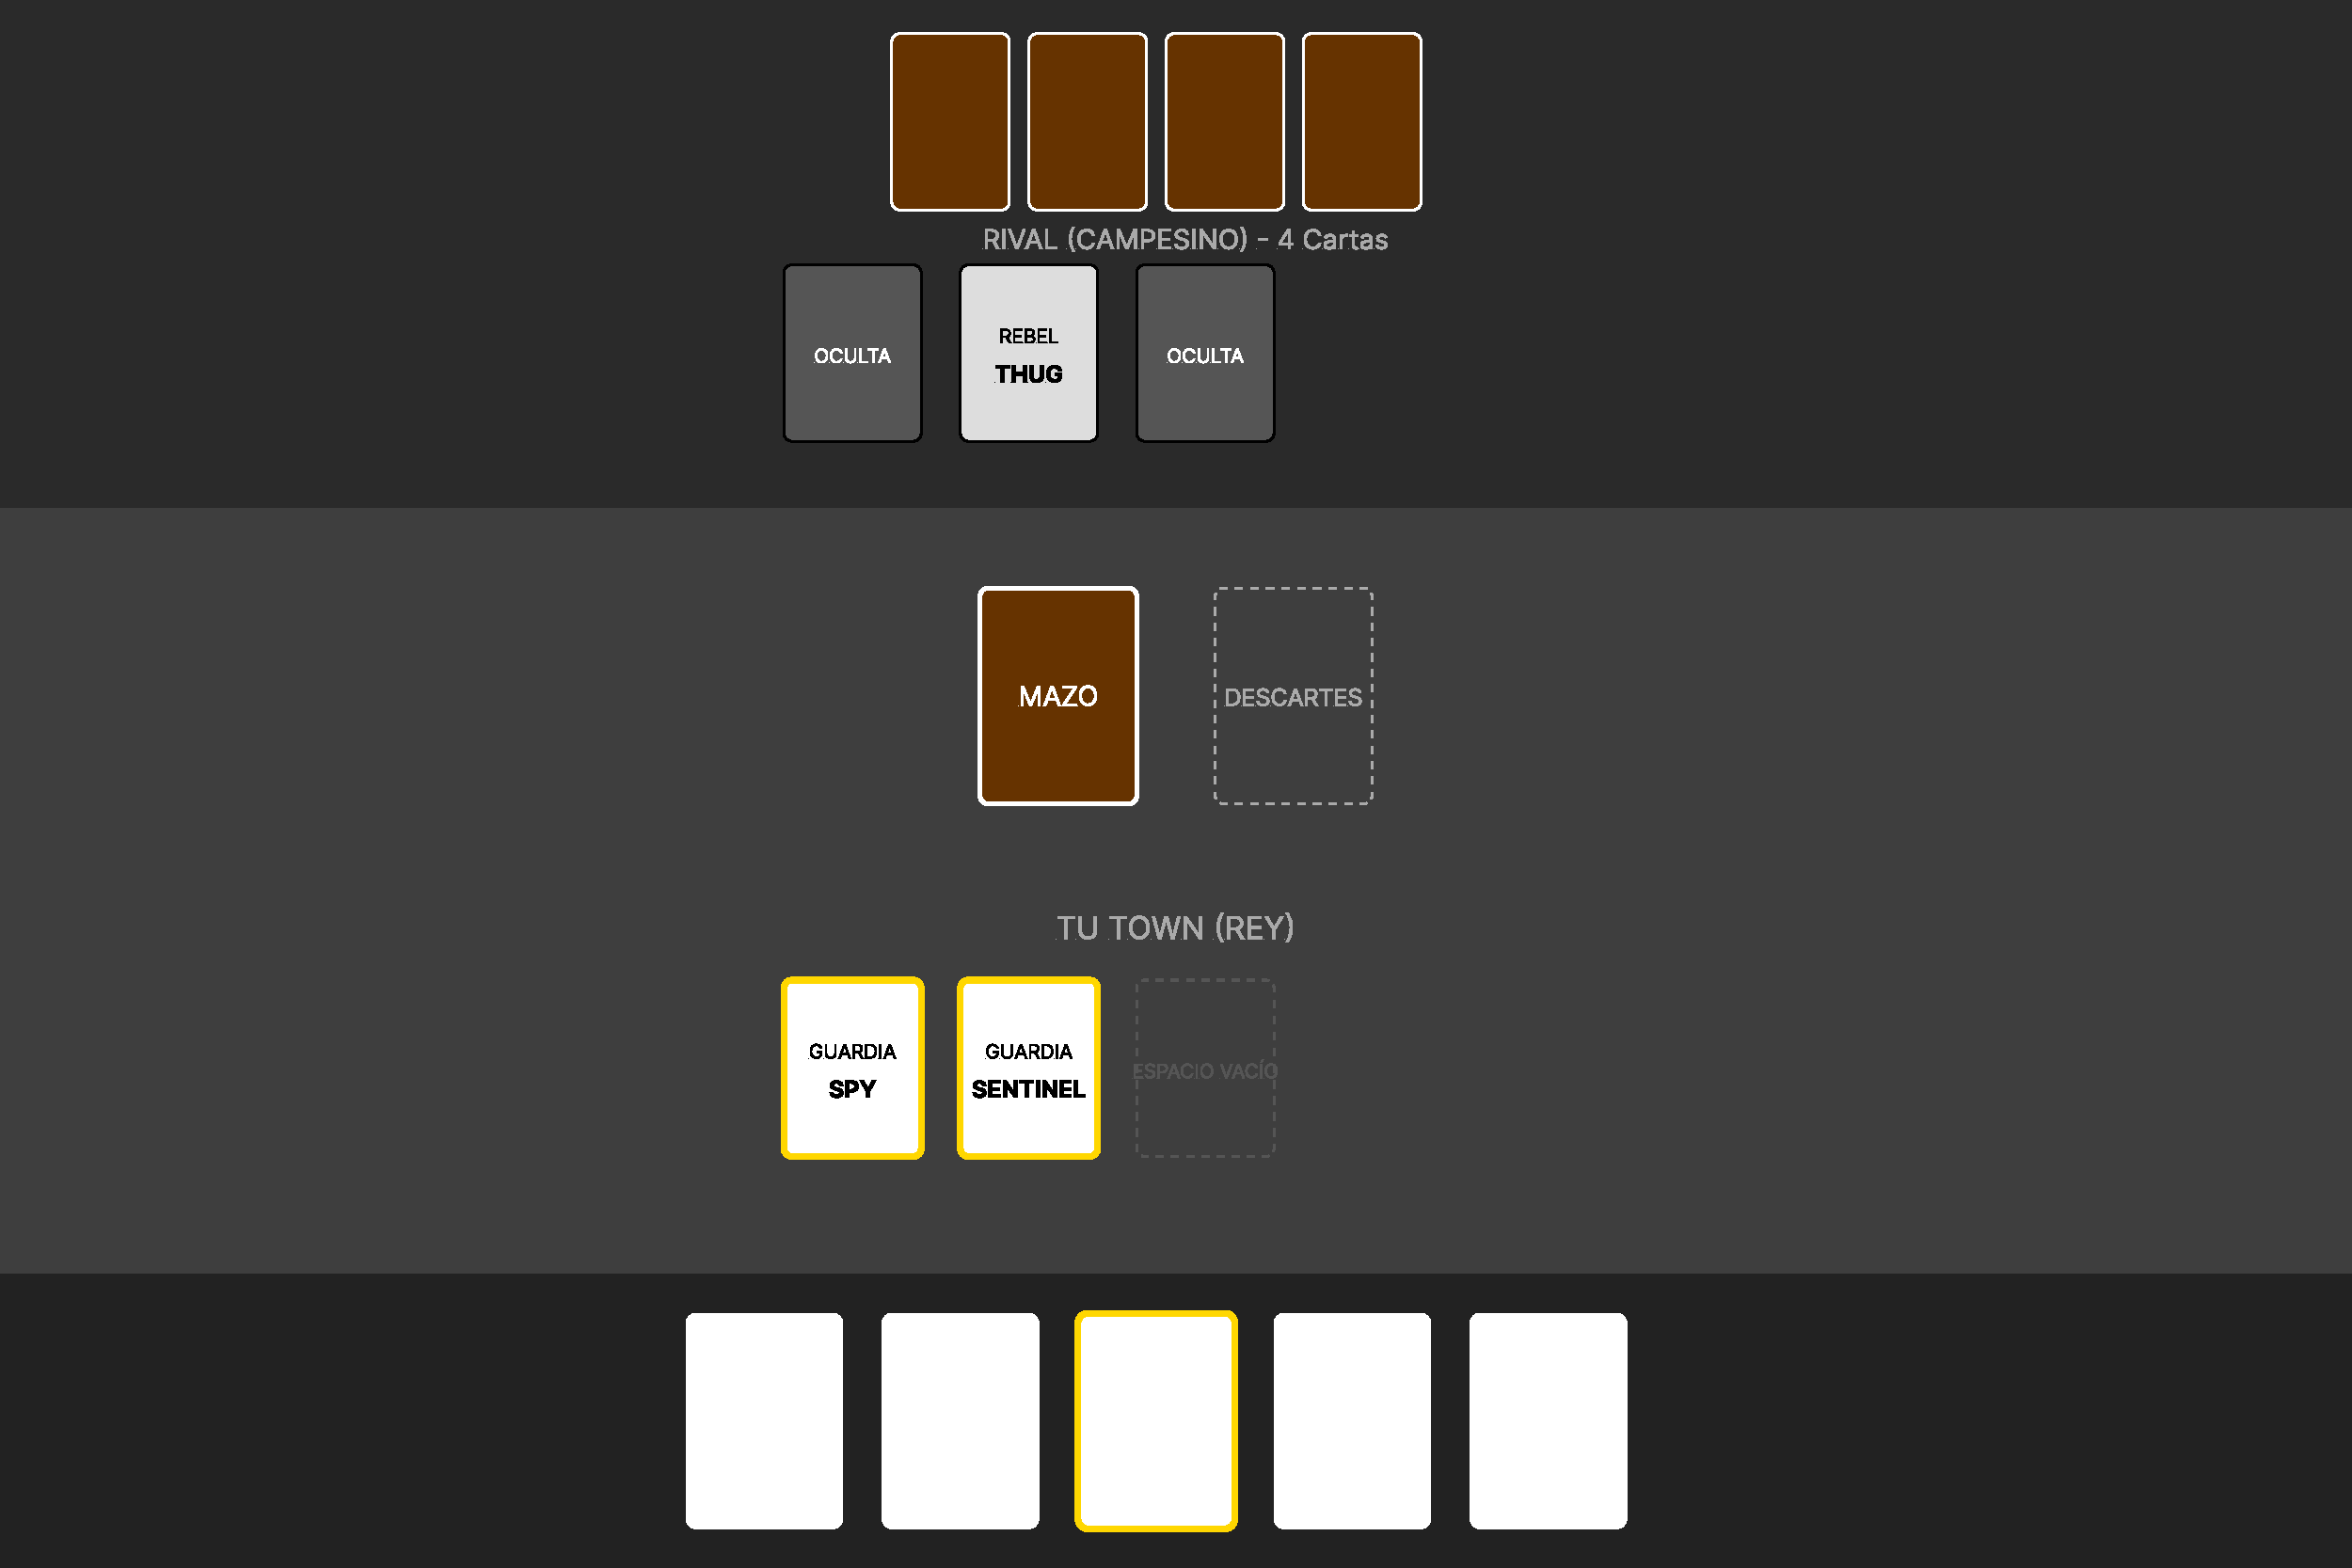
\includegraphics[width=0.9\textwidth]{figures/game_board_ui.pdf}
\caption{Captura de los mock-ups de la interfaz principal: Tablero de juego asimétrico y salas de espera (Lobbies).}
\label{fig:ui_gameboard}
\end{center}
\end{figure}

Se diseña un entorno de pruebas híbrido utilizando Jest para validar la lógica del servidor (\textit{backend}) y Vitest para los componentes de la interfaz de usuario (\textit{frontend}). Para el despliegue de la aplicación, se opta por la plataforma Render debido a su integración nativa con entornos Node.js. La elección de este servicio se fundamenta en la disponibilidad de un plan gratuito y en que se dispone de experiencia técnica previa en su configuración, lo que facilita la gestión de la infraestructura. El flujo de CD se diseña para activarse automáticamente mediante GitHub Actions cada vez que se integren cambios en la rama principal y en la rama \textit{trunk}.

\section{Detalles de Implementación}
La integración de múltiples motores de bases de datos exige un desarrollo cauteloso en el archivo \texttt{docker-compose.yml}. Se implementan volúmenes persistentes (\textit{Volumes}) tanto para \textit{MariaDB} (\texttt{/var/lib/mysql}) como para \textit{Redis} (\texttt{/data}), asegurando que la reinicialización de los contenedores no provoque la pérdida de información crítica. Adicionalmente, se ejecutan comprobaciones de estado (\textit{healthchecks}) con comandos nativos como \textit{mysqladmin ping} y \textit{redis-cli ping}, garantizando que los servicios de \textit{backend} dependientes (\textit{depends\_on}) no intenten establecer conexiones hasta que los motores estén operativos.

En cuanto al sistema de pruebas, se procede a la instalación y configuración de las librerías de testeo en ambos paquetes del monorepositorio.

De cara al despliegue, se implementa un flujo de trabajo automatizado para el despliegue. Este \textit{workflow} actúa como un puente entre el repositorio de código y el servidor de producción; se encuentra configurado para activarse ante dos eventos: la publicación de una nueva versión (\textit{release}) o la realización de un \textit{push} en la rama \texttt{trunk}. 

Al dispararse, el proceso se ejecuta en una máquina virtual con Ubuntu que realiza una petición HTTP POST mediante la herramienta \texttt{curl} a un \textit{webhook} específico de Render. La dirección de este enlace se gestiona de forma segura a través de los secretos del repositorio (\textit{secrets}) para evitar accesos no autorizados. Al recibir esta señal, Render inicia automáticamente la construcción de la nueva versión, instalando las dependencias necesarias y actualizando el servicio en la nube. Asimismo, durante la integración del almacenamiento en memoria, surgieron bloqueos temporales en la comunicación de los servicios locales. Este problema técnico se solucionó en caliente corrigiendo el mapeo de puertos y exponiendo explícitamente el puerto 6379 hacia el \textit{localhost} dentro de la configuración del archivo \texttt{docker-compose.yml}.

\section{Seguimiento, Control y Replanificación}
Durante el seguimiento de esta fase se identifica una desviación significativa respecto a la planificación temporal. La decisión de configurar el entorno de despliegue de manera prematura, sin contar todavía con código funcional de la aplicación para validar el proceso de extremo a extremo, generó un consumo de tiempo mal distribuido. Al haber invertido este esfuerzo de forma anticipada, sumado al tiempo dedicado a resolver los conflictos de red mencionados en la implementación, la iteración se vio retrasada respecto a lo previsto inicialmente.

Como medida de replanificación, será necesario realizar un esfuerzo mayor durante las iteraciones futuras para compensar este retraso y lograr cuadrar el cronograma general. Además, la validación definitiva de la subida a producción queda obligatoriamente pospuesta para la iteración 16 (fase de despliegue final), momento en el que el sistema ya contará con la base de datos poblada y el flujo automatizado completo que justifiquen la prueba en la red. A nivel de trazabilidad de progreso, este ciclo concluye certificando el cierre de la tarea 1.2 (Contenedorización mediante Docker), quedando la tarea 1.3 (Flujos de Integración Continua) pendiente y arrastrada en el calendario.
